\documentclass{article}
\usepackage[utf8]{inputenc}
\usepackage{amsmath}
\usepackage{amsfonts}
\usepackage{amssymb}
\usepackage{blindtext}
\usepackage{biblatex}
\usepackage{graphicx}
\title{Project 1}
\author{Espen Ulset Nordsveen
\and Ghadi Al Hajj}
\begin{document}
\maketitle
\section{Introduction}
Linear regression is an important tool within the field of statistics and data analysis. This statistical method aims to determine the strength and character of the relationship between one dependent variable, also called the outcome, and one or more independent variables, also called the features. This is achieved by mapping this relationship through a mathematical formula that best approximates the data points within a given data set.

This tool is used in several fields of science spanning medicine, physics, finance, astronomy...

In this project, our goal was to analyse and compare the performance of various linear regression methods, namely the Ordinary Least Squares (OLS), Ridge regression and the Lasso regression. These methods were combined with resampling techniques like the bootstrap and cross validation techniques to get better estimates of the error, specifically on the test data. In addition, bootstrap was used to perform a bias-variance tradeoff analysis for all methods.

\subsection{Linear Regression}
As mentioned, linear regression attemps to find a relationship between two or more variables by fitting a linear equation to observed data. We denote the dependent variable, or outcome, as $\textbf{y}$. If we have a set of independent variables, or features, $\textbf{X}^{T} = (X_{1}, X_{2}, \dots, X_{p})$, and assuming a linear relationship between these, the $y$ can be predicted as
\begin{equation} \label{ytilde}
\tilde{y} = \tilde{\beta_{0}} + \sum_{j=1}^{p} X_{j} \tilde{\beta_{j}}
\end{equation}
By including the constant variable 1 in $X$, and include $\tilde{\beta_{0}}$ in the vector of coefficients $\tilde{\beta}$,  (\ref{ytilde}) can be written in vector form as
\begin{equation}
\textbf{y} = \textbf{X} \beta + \epsilon
\end{equation}
where $\epsilon$ denotes the residual error of the linear model $\textbf{X}\beta$ from the true response, and the $\beta$ is the parameter vector containing the linear regression coefficients $\beta_{i}$. $y$, $\textbf{X}$ and $\epsilon$ are defined as the following vectors
\begin{equation}
\textbf{y} = [y_{0}, y_{1}, y_{2}, \dots, y_{n-1}]^{T}
\end{equation}

\begin{equation}
\beta = [\beta_{0}, \beta_{1}, \beta_{2}, \dots, \beta_{n-1}]^{T}
\end{equation}

\begin{equation}
\epsilon = [\epsilon_{0}, \epsilon_{1}, \epsilon_{2}, \dots, \epsilon_{n-1}]^{T}
\end{equation}
and $\beta$ are in fact the unknown parameters in the linear regression problems that needs to be calculated.
\begin{equation}
\textbf{\~{y}} = \textbf{X}\beta + \epsilon
\end{equation}

The design matrix
\begin{equation} \label{designM}
\textbf{X} = 
\begin{bmatrix}
1 & x_{0}^{1} & x_{0}^{2} & \dots & x_{0}^{n-1} \\
1 & x_{1}^{1} & x_{1}^{2} & \dots & x_{1}^{n-1} \\
1 & x_{2}^{1} & x_{2}^{2} & \dots & x_{2}^{n-1} \\
\vdots & \vdots & \vdots & \dots & \vdots \\
1 & x_{n-1}^{1} & x_{n-1}^{2} & \dots & x_{n-1}^{n-1} \\ 
\end{bmatrix}
\end{equation}

\subsection{Ordinary Least Squares}
\begin{equation}
C(\textbf{X},\beta) = \dfrac{1}{n} \{( \textbf{y}-\textbf{X}\beta^{T}\textbf{y}-\textbf{X}\beta)\}
\end{equation}
\subsection{Ridge Regression}
\begin{equation}
C(\textbf{X},\beta) = \dfrac{1}{n} \{( \textbf{y}-\textbf{X}\beta^{T}\textbf{y}-\textbf{X}\beta)\} + \lambda \beta^{T} \beta 
\end{equation}
\subsection{Lasso Regression}
\subsection{The bootstrap}
The boostrap resampling method is a simple Monte Carlo technique to approximate the sampling distribution (KILDE). The method randomly draw $B$ datasets with replacement from the training data, where each sample is the same size as the original training set. The model is then refit to the $B$ bootstrap datasets. In the context of this project, we use this method to calculate MSE, bias and variance of the model.
\subsection{k-fold Cross Validation}
The $k$-fold Cross Validation technique is a resampling procedure used to evaluate the performance of statistical models on a limited data sample. The method generally results in a less biased or less optimistic estimate of the model compared to other methods, such as the train/test split. The \textit{k} refers to the equally number of groups the given sample shall be split into. One of these groups are set aside as the validation group. The rest of the groups, i.e. $K-1$, are used to fit the model, and calculate the prediction error of the fitted model when predicting the $k$th part of the data. A normal value for $k$ is $K=5$, as this gives a lower variance. It might, however, give problems with the bias if the training sets becomes too small.

The general procedure for the $k$-fold Cross Validation is as follows (KILDE)
\begin{enumerate}
\item Shuffle the dataset
\item Split the dataset into $k$ groups
\item For each unique group
\begin{enumerate}
\item Take the group as a hold out or test data set
\item Take the remaining groups as a training data set
\item Fit a model on the training set and evaluate it on the test set
\item Retain the evaluation score and discard the model
\end{enumerate}
	
\item Summarize the skill of the model using the sample of model evaluation scores
\end{enumerate}

\section{Data}
\subsection{Franke's function}
The Franke's function will be used as a basis for our discussion of the various regression and resampling methods in this context. This is a function  widely used as a test function in interpolation problems.

\begin{align*}
f(x,y) &= \frac{3}{4}exp\left(-\frac{(9x-2)^2}{4} - \frac{(9y-2)^2}{4}\right)+\frac{3}{4}exp\left(-\frac{(9x+1)^2}{49} - \frac{(9y+1)}{10}\right)\\
&+ \frac{1}{2}exp\left(-\frac{(9x-7)^2}{4} - \frac{(9y-3)^2}{4}\right)-\frac{1}{5}exp\left(-(9x-4)^2 - (9y-7)^2\right)
\end{align*}
\section{Method}
The Franke function is a multivariable function, depending on both $x$ and $y$, and hence is a 2-variable polynomial. The design matrix in \ref{designM} thus needs to be adjusted for this multivariable case. The 
$$\textbf{X} = \begin{bmatrix}
1 & x_{0} & y_{0} & x_{0}y_{0} & \dots & x_{0}^{N} & y_{0}^{N}     \\
1 & x_{0} & y_{1} & x_{0}y_{1} & \dots & x_{0}^{N} & y_{1}^{N}  \\
\vdots & \vdots & \vdots & \vdots & \dots & \vdots & \vdots \\
1 & x_{1} & y_{0} & x_{1}y_{0} & \dots & x_{1}^{N} & y_{0}^{N} \\
\vdots & \vdots & \vdots & \vdots & \dots & \vdots & \vdots \\
1 & x_{n-1} & y_{m-1} & x_{n-1}y_{m-1} & \dots & x_{n-1}^{N} & y_{m-1}^{N} \\
\end{bmatrix}$$
\section{Results}
\subsection{Ordinary least squares on the Franke Function}
In this part, we performed the plain OLS regression on the data that is generated using the Franke function. Before that, we split the data into training set, on which the model is trained, and a testing sets, on which the model’s performance is evaluated for the goodness of the fit. The ratio of training to testing sets 70/30.

For performing the OLS, a polynomial of degree five was used to generate the features of the model, and then these features were scaled according to the training data statistics, in order to force the data into a distribution with zero mean and unit variance. This is useful because it ensures that each feature gets an equal chance of being represented in the polynomial, thus preventing features with large values to dominantly control the shape of the polynomial.

The metrics were then applied to both sets and the R2 coefficient and the Mean Square Error of each set were calculated. In addition, we generated a plot of the confidence intervals of the tunable parameters, shown in figure \ref{fig:confint}.

The Mean Square error was calculated by
\begin{equation}\label{mse}
MSE(y,\tilde{y}) = \dfrac{1}{n}\sum_{i=0}^{n-1} (y_{i} - \tilde{y}_{i})^{2}
\end{equation}
and the R2 coefficient was calculated by
\begin{equation}\label{r2}
R^{2}(y,\tilde{y}) = 1 - \dfrac{\sum_{i=0}^{n-1} (y_{i} - \tilde{y}_{i})^{2}}{\sum_{i=0}^{n-1} (y_{i} - \overline{y}_{i})^{2}}
\end{equation}
where $\overline{y}$ is defined as
\begin{equation}
\overline{y} = \dfrac{1}{n} \sum_{i=0}^{n-1} y_{i}
\end{equation}
\begin{figure}
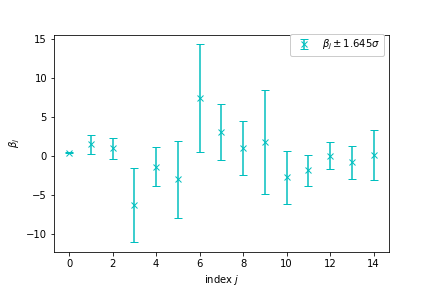
\includegraphics[scale=0.5]{confidenceintervall.png}
\centering
\caption{Confidence intervall of the tunable paramteres}
\label{fig:confint}
\end{figure}

In our demonstration, we noticed that if the design matrix is created from data points within the range of [0,1], then the resulting  matrix would be close to singularity, and the program would thus raise an error whenever the inverse is calculated, particularly when calculating  or its variance. This, in turn, caused the problem of getting negative values for the variance of some values. Using pinv, however, instead of inv, solved both problems when calculating the inverses.

It is also worth mentioning that when the range of values that the raw features can take is increased to, say, [0,5], instead of [0,1], the problem of singular matrices immediately disappears even when using inv and the determinant of the matrix  becomes greater than zero.

\subsection{Bias-variance trade-off and resampling techniques}
When evaluating the model’s performance on the test data that the model has not seen before, we want to measure the difference/error between the model’s predictions and the true values. This error can be split into three terms.

The bias term is a quantity that describes how much the data is shifted from the mean value of the model. A high bias indicates that the model is not able to represent the patterns in the underlying data.

Variance, on the other hand, represents the variance of the predicted data from its corresponding mean, and it describes the sensitivity of the model to the noise in the data. Thus, high variance indicates that the model has not only learned the underlying model, but went further to even capture the noise in the data.

A model that is simple and does not capture the underlying trends in the data is called an underfitting model, and has high bias and low variance. On the other hand, a model that is too complex will likely result in overfitting, in which case it would have low bias and high variance.

Last is the irreducible error term. This represents the error that is not related to the complexity of the model and that cannot be reduced no matter how good and tuned the model is, with a given set of predictors. This error term is given by the variance of the noise in the data, and can be reduced by recognizing more independent predictors that are also related to the dependent variable.

Figure \ref{fig:plot} (add figure for bias variance tradeoff) shows the trends in the bias and the variance as a function of the model’s complexity. 

As expected, at low degrees of complexity, the model suffers from under-fitting as a low order polynomial cannot reasonably represent a complex function with exponential and quadratic terms. This is shown by the high bias for polynomials of low order.

As the complexity increases, the bias starts decreasing indicating that the model is no longer deficient of approximating the overall shape and trends in the data. At a certain polynomial degree (5), the model reaches a balance between bias and variance, where the overall error is the lowest. Such a model is a model that has learned the trends in the data but has not yet entered the stage of memorizing the training data and adapting itself to the noise/idiosyncrasies in the training data.

When the polynomial degree exceeds 5, the variance starts to increase in value indicating that the model has now entered into the realm of over-fitting. This variance will keep increasing as the complexity increases until the model has learned all the noise in the training data. This additional learning negatively impacts the model’s performance on new data and inhibits its ability to generalize to the domain of interest, which is the ultimate goal of any machine learning algorithm.

\begin{figure}
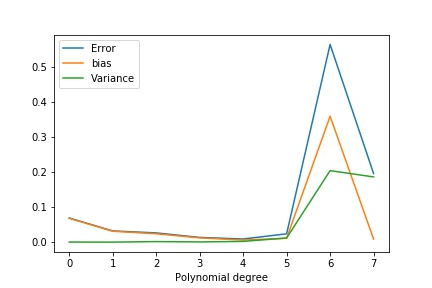
\includegraphics[scale=0.5]{partBplot.jpg}
\centering
\caption{Plot}
\label{fig:plot}
\end{figure}

\begin{figure}
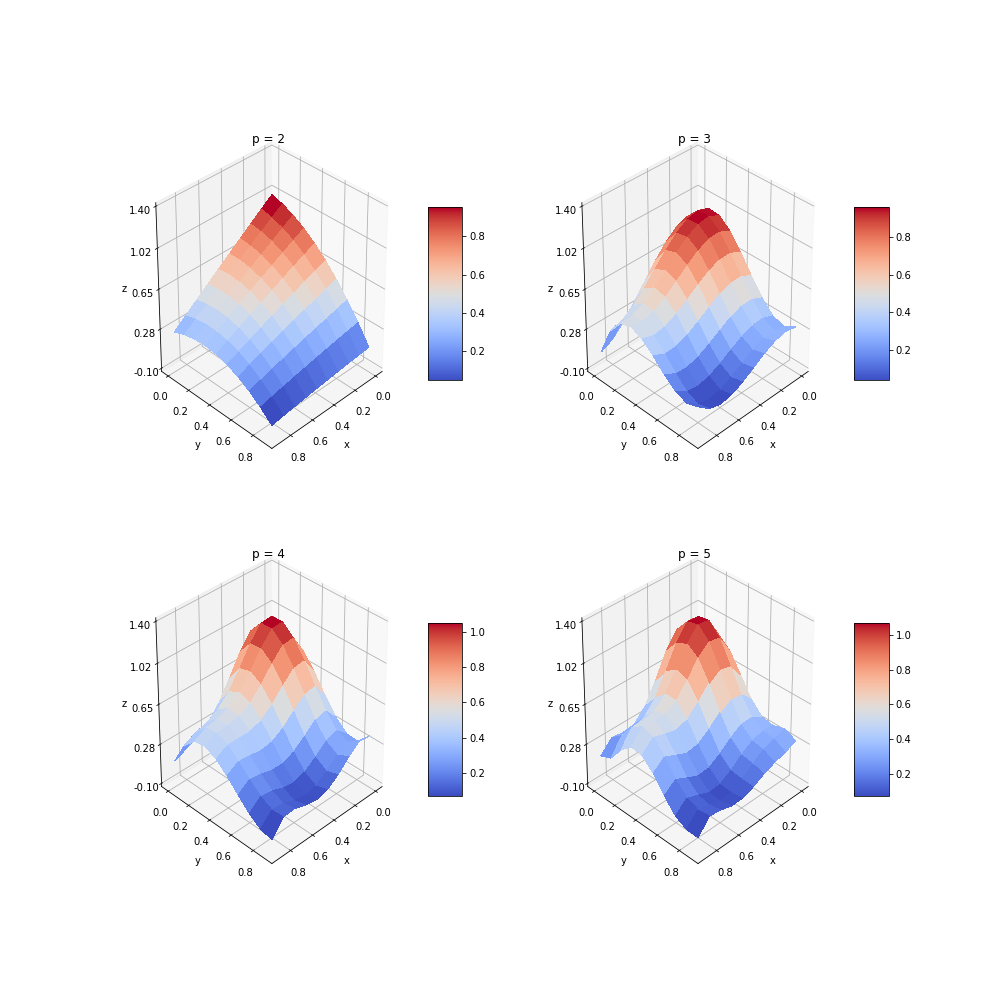
\includegraphics[scale=0.35]{frankePlots.png}
\caption{OLS on the Franke function, with increasing polynomial degree}
\end{figure}

\subsection{Cross-validation as resampling techniques}
In this part, we performed a k-fold cross validation analysis to estimate the value of the Mean Square Error of our model of a seventh degree polynomial. We estimated this quantity using 5 and 10 folds.

The cross validation analysis gives estimates of 0.0033 and 0.0021, for 5- and 10-folds, respectively, which are both relatively lower than the estimate of this quantity from bootstrap at the same model complexity, 0.1019. This illustrates the fact that cross validation gives an over optimistic estimate for this error.

It is also important to note that the bootstrap approach is closer to the real scenario because after each bootstrapping iteration, the model is tested on the same test set, whereas in cross validation, each time the test set is changed.


\subsection{Ridge regression}
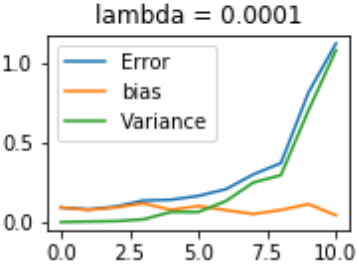
\includegraphics[scale=1]{boostrapridge0.png}
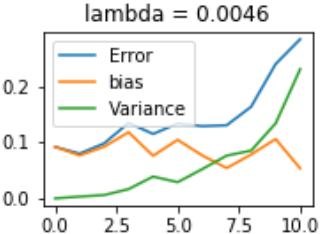
\includegraphics[scale=1]{boostrapridge1.png}

\subsection{Lasso regression}

\subsection{Introducing real terrain data}
\begin{figure}
\begin{minipage}{0.48\textwidth}
\centering
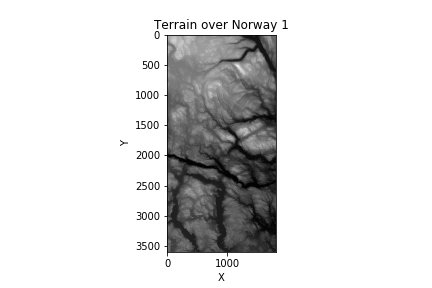
\includegraphics[width=1.5\linewidth]{terrain2dplot.png}
\end{minipage}
\begin{minipage}{\textwidth}

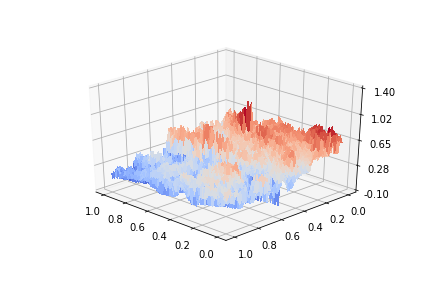
\includegraphics[width=0.7\linewidth]{rawdataplot.png}
\end{minipage}
\caption{2D and 3D plot of the terrain data used as basis for our analysis}
\end{figure}



\subsection{Regression techniques on terrain data}
\end{document}

